\chapter*{Data acquisition}
A part of this master's thesis involves creating a knowledge base that includes certain queryable parameters, allowing the robot to perform specific actions. The initial step in building the knowledge base is to gather data. In this chapter, we elaborate on our data acquisition strategy.
\section*{Task variations}
	As our main focus is to represent the knowledge about mixing, first we had to acquire the different types and variations of mixing in order to create a complete Knowldegerepresentation. The first step in acquiring the needed data, was to acknowledge which task varations of mixing are actually important. 
  So we had to analyze the word \textit{Mixing} and its hyponyms. But first we have to ask ourselves What is Mixing?
  \subsection*{What is Mixing?}
  The definition provided by the Oxford Dictionary is as follows: To put together or combine (two or more substances or things) so that the constituents or particles of each are interspersed or diffused more or less evenly among those of the rest; to unite (one or more substances or things) in this manner with another or others; to make a mixture of, to mingle, blend.
  Ultimately, this definition conveys that mixing requires at least two elements or substances, which are then combined (evenly) with each other, resulting in a (new) substance.
  This definition is general and can be applied to various contexts. For our work, the aspect of cooking or mixing different (cooking) ingredients is important. Therefore, we consider some hyponyms of the verb "mixing" irrelevant for our cause and do not take them into account.
  An adapted definition for our work could be: Mixing is the combination of various (cooking) ingredients through different motions in a container.
  
  \subsection*{Mixing hyponyms analysis} 
	Hyponyms are subordered words of a given word, for example one hyponym of mixing could be beating. 
  To conduct this analysis, one can utilize tools from various websites, such as FrameNet and WordNet. These platforms provide users with the ability to search for specific words and obtain various associations for those words, including synonyms, acronyms, or, crucial for our case, hyponyms.	
  For all those hyponyms, we delegated a WikiHow extraction search which should show us, how many times one of these words occur, in the context of cooking.
	In the table below the results can be seen.
	
    \begin{table}[H]
        \centering
        \begin{tabular}{|c|c|}
          \hline
          \textbf{Hyponym} & \textbf{Occurance}  \\
          \hline
          Mixing & 5300 \\
          \hline
          Combining & 3700  \\
          \hline
          Stirring & 6810 \\
          \hline
          Folding & 970 \\
          \hline
          Merging & 7 \\
          \hline
          Beating & 1200 \\
          \hline
          Whipping & 1000 \\
          \hline
          Join & 57 \\
          \hline
          Coalesce & 1 \\
          \hline
          Amalgamate & 0 \\
          \hline
          Pair & 57 \\
          \hline
          Blending & 1400 \\
          \hline
    
        \end{tabular}
        \caption{Example Table}
        \label{tab:example}
      \end{table}
      

	From this table one can see that many hyponyms have a low occurance and will be therefore not considered.
	We consider the words: Mixing, Stiring, Beating, Combining, Whiping, Whisking and Folding. Though Blending achieved a moderate occurance, we decided upon not considering it, because it involves a lot of electronic mixing machines, which the robot could not handle.
	From now on we will refer to these words also as Tasks.

  \section*{Task definitions}
  After selecting our tasks, we need to analyze the context in which they are used. To achieve this, we primarily analyzed WikiHow and various (cooking) videos that include at least one of the tasks we selected. The analysis revealed that the various tasks are primarily used in different contexts, leading to different motions. Additionally, we could conclude that each action involves the following components:	
	\begin{itemize}
		\item Tasks: The tasks can differ in its execution, like the tasks Beating (Mixing can be gentle or vigorous, while beating involves a more forceful and rapid action) and Folding (To maintain a light and fluffy texture in a cake, folding is often used to add dry ingredients without overmixing), which will ultimately lead to a decision upon which Motion should be used in the specific use case.
		\item Tools: Different Tools are used for different tasks, which also has a correlation with the choosen Container.
		\item Container: Most Mixing Tasks use a mixing bowl for container, but also container like Pot and Pan when considering cooking in boiling water.
		\item Ingredients: Besides Tasks, the ingredients are the most important component of our knowledgebase regarding the decision making upon motions. We divide the Ingredients in 4 subcategories: Dry/Powder, Wet, Liquid and Solid.
		\item Motions: The motions used in the analyzed videos will help us upon creating a knowledgebase from which the robot should be able to infer which motions he will use in different situations.
	\end{itemize}
  \subsection*{Concluded Motions from video analysis}
	In the following we want to present our analysis results regarding the videos from WikiHow, but also from well known cooks, like Jamie Oliver:


    \begin{table}[H]
        \centering
        \begin{tabular}{|c|c|c|p{4,5cm}|p{4,5cm}|}
            \hline
            \textbf{Task} & \textbf{Tool} & \textbf{Container} & \textbf{Ingredients} & \textbf{Description} \\
            \hline
            Beating & Whisk & Bowl & Egg yolk (Wet ingredient) & circular, swirling wildly around the bowl \\
            \hline
            Stirring & Whisk & Bowl & Beaten Egg Yolk (Wet), Parmesan(Powder) and Pepper (Powder) & Circular, from the inside to the outside. \\
            \hline
            Stirring & Tongs & Pan & Wet Mixture, Pasta (Solid) and Bacon (Solid) & Diving motions, circular but also straight lines. \\
            \hline
            Whisk & Fork & Bowl & Eggs (Wet) & Circular but also straight, wildly motion. \\
            \hline
            Mixing & Spatula & Pan & Eggs, melted butter (Wet) & Circular, from the inside to the outside, also diving. \\
            \hline
            Folding & Spatula & Pan & cooked eggs in melted butter (Wet) & Gently motion from the outisde to the inside straight, then moving about 90 degree before going to the inside again. \\
            \hline
            Mixing & Spoon & Cup & Dry yeast(Powder), Water (Liquid) & Circular \\
            \hline
            Mixing & Spoon & Bowl & Dry yeast, Water, Flour (Powder), Salt(Powder) & Whirlstorm-like motion. \\
            \hline 
        \end{tabular}
        \caption{Example Table}
        \label{tab:example}
      \end{table}
      

	From this videos we extracted informations about the executed motions. The following motions can be defined:
	\begin{itemize}
		\item \textbf{Circular}: Moving the tool in a defined circular movement in the container, not changing the radius during execution
		\item \textbf{Whirlstorm}: Moving from the inside to the outside of the container with the tool, by circulating in an incremented radius.
		\item \textbf{Folding}: Gently motion, where you start from the outside, moving one straight line to the inner side, then picking the tool up and going to the initial state before moving the tool for about 90 degrees, then going back in a straight line to the inner side of the container again.
		\item \textbf{VerticalCircular}: Imagine a line which can be seen as the diameter of the container, from this line one can define certain regions on which you move the tool circular from side to side. This motion is used by the beating task.
		\item \textbf{CircularDivingToInner}: Starting from the outerside, moving the tool in the container arround its edge for about 270 degrees, before diving to the middle of the container. This motion is used by Tasks where is required to turn the Ingredients over.
	\end{itemize}

	By analyzing the videos we concluded that the motion decision is based on the task and Ingredients. Upon this thoughts we decided to design a decision tree regarding how the motions will be choosen by the robot.
\newpage
\section*{Decision Trees}
In this section we want to illustrate the decision tree for the ellaborated tasks, starting with the Mixing task.
This trees should decide which motion is used for given Task and Ingredients combinations, as well as which Tool and Container would be preffered.
For example if we regard the combination of: \newline Task: Mixing + Ingredients: Wet and Liquid -> WhirlstormMotion. The preffered Container would be the bowl, and the preffered tools would be the spoon and whisk.
Some Tasks do not contain every possible Ingredients combinations, so the Decision Trees might be uncompleted. We also regard the Combining task eqully to the Mixing task.

\subsection*{Mixing}
\begin{figure}[H]
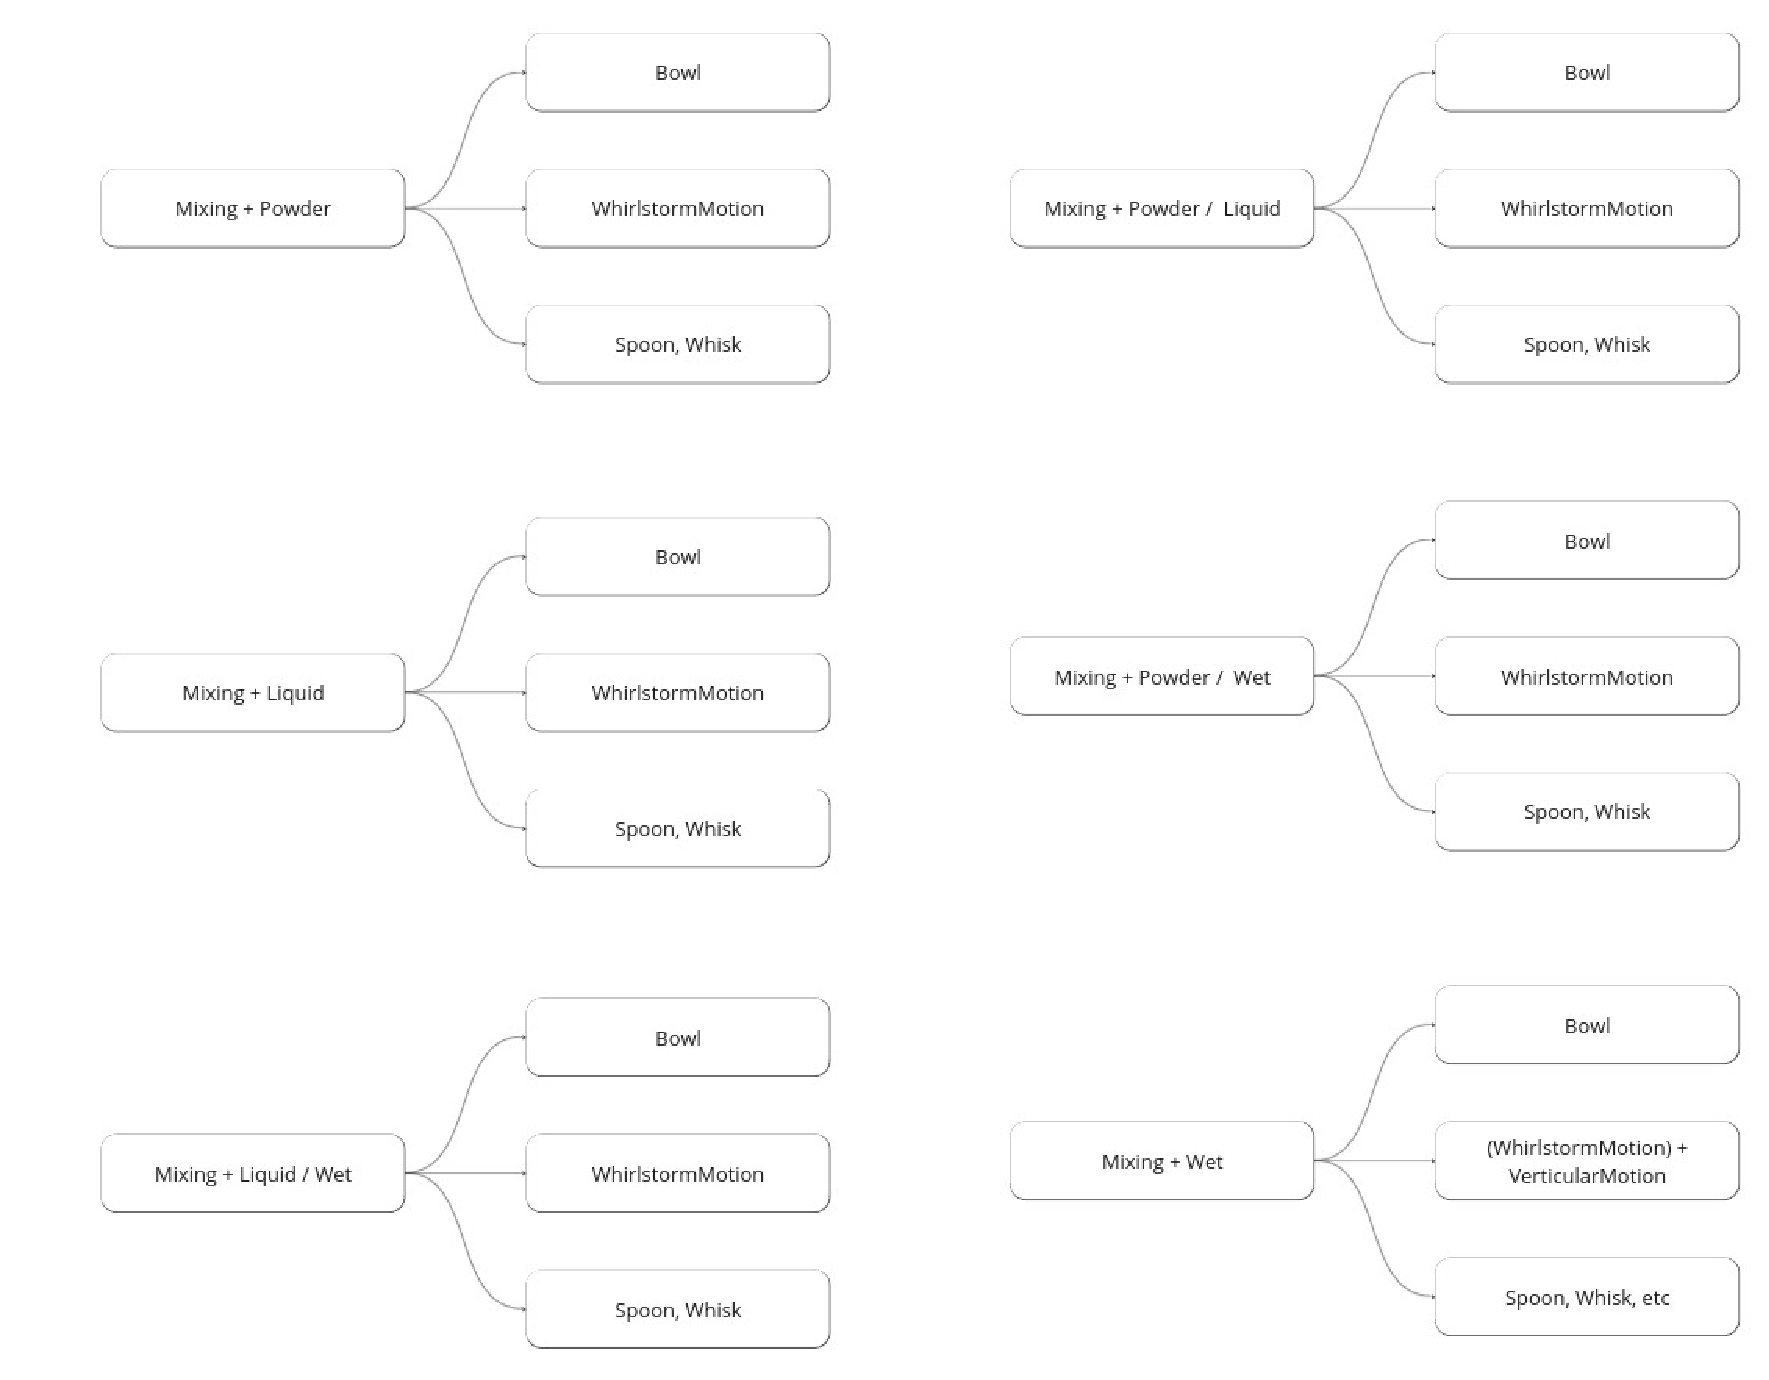
\includegraphics[scale=0.5]{Graphics/MixingDT.pdf}
\end{figure}

\subsection*{Stiring}
\begin{figure}[H]
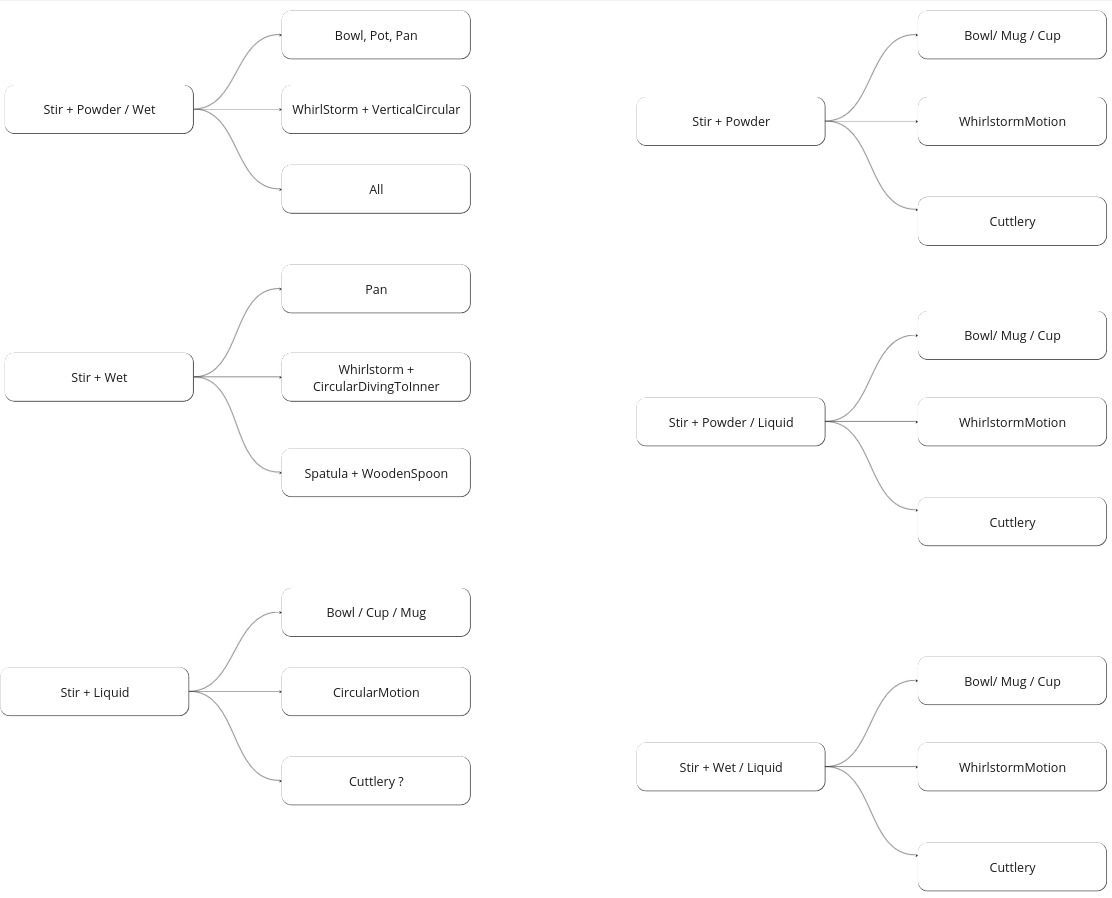
\includegraphics[scale=0.4]{Graphics/StirringDT.jpg}
\end{figure}


\subsection*{Beating}
\begin{figure}[H]
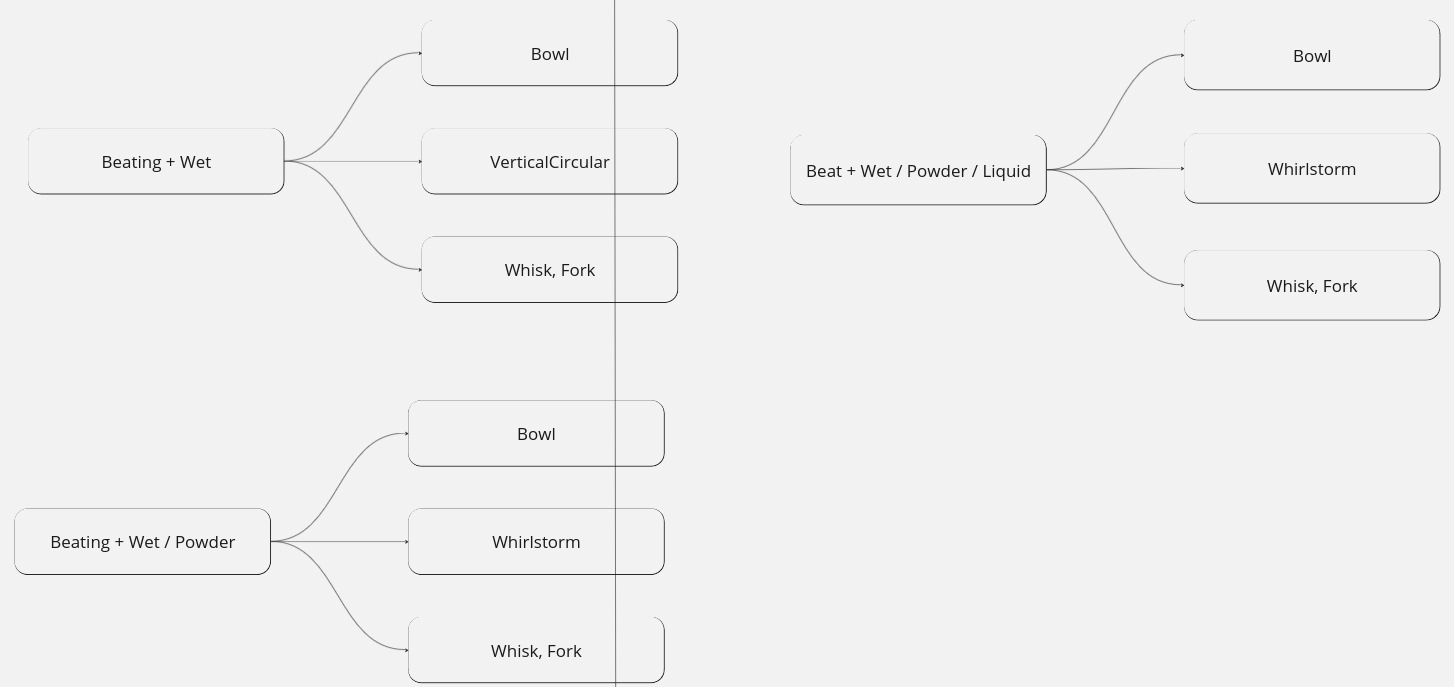
\includegraphics[scale=0.3]{Graphics/BeatingDT.jpg}
\end{figure}

\subsection*{Whisking}
\begin{figure}[H]
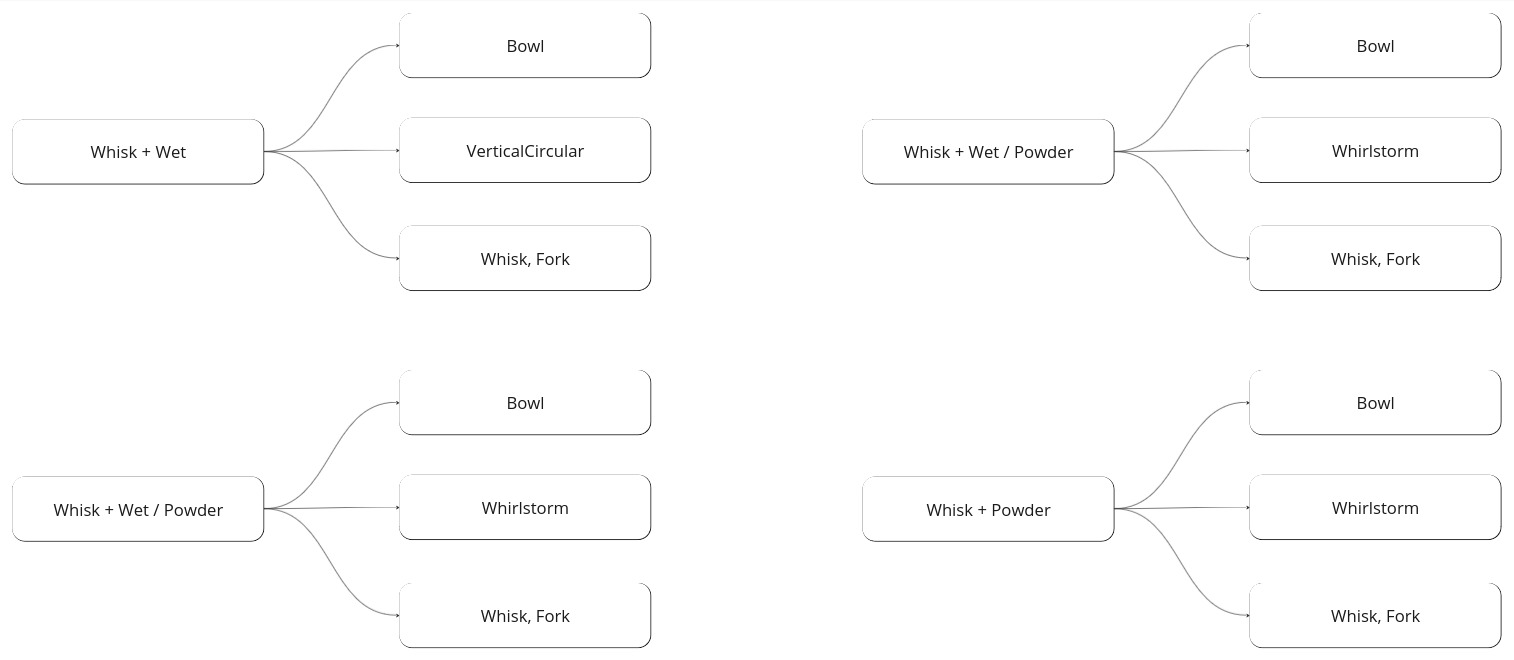
\includegraphics[scale=0.3]{Graphics/WhiskingDT.jpg}
\end{figure}